\section{Recolección de datos}

\begin{frame}{Recolección de datos}
    \begin{itemize}
        \item Aún teniendo un modelo válido, si los datos se recogen de una manera inadecuada, o son analizados incorrectamente, los resultados del modelo serán erróneos y pueden conducir a malas decisiones.
        \item Hay riesgos derivados de la escasez de datos disponibles, o de datos irrelevantes, desactualizados o simplemente erróneos.
    \end{itemize}
\end{frame}


\begin{frame}{Recolección de datos}
    \begin{itemize}
        \item Algunas sugerencias para la recolección de datos son:
    \begin{itemize}
        \item Planeación: observación del sistema actual y situaciones atípicas.
        \item Análisis de los datos a medida que son recolectados.
        \item Verificar homogeneidad en los diferentes grupos de datos.
        \item Revisar la relación entre variables.
        \item Revisar autocorrelación.
        \item Diferenciar claramente entre datos de entrada y de salida.
    \end{itemize}
    \end{itemize}
\end{frame}


\begin{frame}{Modelos de entrada sin datos}
    \begin{itemize}
        \item Si el sistema a modelar No existe, el analista debe confiar en datos más vagos, que pueden incluir:
        \begin{enumerate}
            \item Experiencias previas.
            \item Opinión de expertos.
            \item Intuición.
            \item Conjeturas a partir de las limitaciones físicas, datos de ingeniería, estándares o la naturaleza del proceso.
        \end{enumerate}
    \end{itemize}
\end{frame}

\begin{frame}{Modelos de entrada sin datos}
    \begin{itemize}
        \item En muchas aplicaciones de la vida real, se utilizan heurísticas como:
    \begin{itemize}
        \item Variables aleatorias con poca variabilidad se simplifican y modelan como deterministas.
        \item Para distribuciones desconocidas se postulan forma funcionales particulares que incorporen cualquier información disponible (Triangular, Uniforme). 
        \item La experiencia a veces puede proporcionar información sobre la forma funcional de las distribuciones.
    \end{itemize}
    \end{itemize}
\end{frame}

\begin{frame}{Modelos de entrada con datos}
    \begin{itemize}
    \item Si el sistema a modelar ya existe, entonces puede proporcionar los datos empíricos necesarios a partir de mediciones en campo.
    \end{itemize}
\end{frame}

\begin{frame}{¿Qué datos se requieren tomar?}
    \begin{itemize}
        \item Dentro de los datos de entrada a recolectar se requieren aquellos relacionados con tiempos entre llegadas, tiempos de servicio, tiempo a la falla de máquinas/recursos, duración de las fallas, tiempos de desplazamiento, probabilidades de tener ciertos valores de atributos (tipos de cliente, cantidad de demanda).
        \item La recolección de datos de las medidas de desempeño del sistema en estudio también es esencial para la validación del modelo.
        %\item Dichas mediciones empíricas deben recolectarse de forma rutinaria siempre que sea posible con miras a la validación futura.
    \end{itemize}
\end{frame}

\begin{frame}{¿Cuántos datos se requiere tomar?}
    \begin{itemize}
        \item Si $\bar{x}$ es un estimador de $\mu$, se puede tener un $100\left(1-\alpha\right)$\% de confianza de que el error no excederá una cantidad específica $e$ cuando el tamaño de muestra sea:
        \[n=\left(\dfrac{z_{\alpha/2}\times \sigma}{e}\right)^2\]
    \end{itemize}
    \begin{figure}
        \centering
        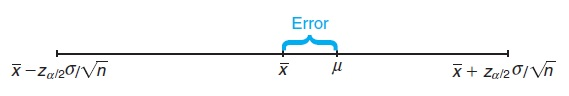
\includegraphics[width=8cm]{images/error_x.jpg}
        %\caption{Caption}
        %\label{fig:my_label}
    \end{figure}
\end{frame}

\begin{frame}{¿Cuántos datos se requiere tomar?}
    \begin{itemize}
        \item Si $\hat{p}$ es un estimador de $p$, se puede tener un $100\left(1-\alpha\right)$\% de confianza de que el error no excederá una cantidad específica $e$ cuando el tamaño de muestra sea:
        \[n=\left(\dfrac{z^2_{\alpha/2}\times \hat{p} \times \hat{q}}{e^2}\right)\]
    \end{itemize}
    \begin{figure}
        \centering
        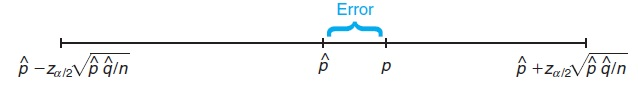
\includegraphics[width=8cm]{images/error_p.jpg}
        %\caption{Caption}
        %\label{fig:my_label}
    \end{figure}
\end{frame}